\documentclass[8pt]{beamer}
\usepackage{amsmath}
\usepackage{amssymb}
\usepackage{graphicx}
\usepackage{hyperref}
\usepackage{color}
\usepackage{float}
\usepackage{subfig}


%\usepackage{sidecap}
\title{Random loops model can explain the appearance of Topologically Associating Domains (TADs)}
\author{Ofir Shukron}
\usetheme{Madrid}
\usecolortheme{dolphin}

\begin{document}

\begin{frame} %{Stochastic Simulation of Topologically Associating Domains}
\titlepage
\end{frame}

\section{Introduction}\label{section_introduction}

\begin{frame}{Introduction}
\begin{enumerate}
\item The spatio-temporal organization of a chromosome has significant implication for nuclear activities, such as gene regulation. 
\item However, the organization of the chromatin is not entirely known.
\item It is known that dynamic packing of the chromatin allows for long range gene regulation.
\item Stable regions in the genome termed TAD, where shown to exist in the population level. 
\item Here we show that using random polymer looping model we can explain the appearance of conserved structures in chromatin called TADs.
\item Given the static interaction maps, what can we say about the underlying dynamical polymer model?
\end{enumerate}
\end{frame}

\begin{frame}{Agenda}
\tableofcontents
\end{frame}

\section{The experimental setting}\label{section_theExperimentalSetting}

\subsection{Chromosome Conformation Capture Carbon Copy (5C)}\label{subsection_chromosomeConformationCaptureExperiments}

\begin{frame}{Chromosome Conformation Capture Experiments}
A set of methods to simultaneously record millions of looping events occurring within the genome. 

The general steps are:
\begin{enumerate}
\item Nuclei are extracted from millions of cells;
\item Formaldehyde induces protein-DNA and protein-protein cross-links;
\item restriction enzymes digest the cross-linked DNA;
\item cross-linked DNA is purified, diluted and ligated;
\item cross-links are reversed;
\item PCR to amplify ligation junctions;
\item The histogram of segments' encounter is produced.
\end{enumerate}
\begin{figure}[H]
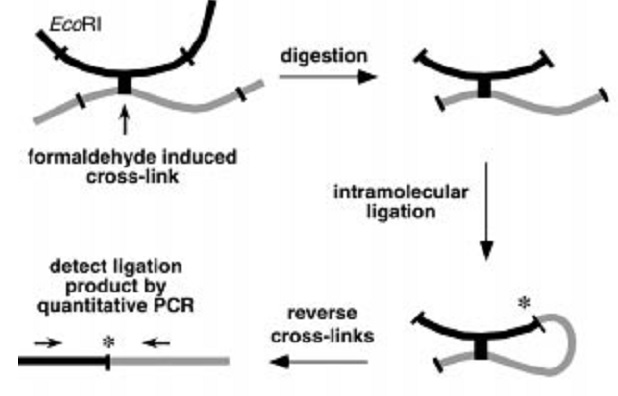
\includegraphics[scale=0.3]{3Cschematic}
\end{figure}
\end{frame}

\subsection{The experimental Data}\label{subsection_theExperimentalData}

\begin{frame}{The experimental data}
\begin{itemize}
\item Two replicate of the 5C experiments were conducted by Nora et. al 2012. 
\item Cells taken from undifferentiated mouse embryonic stem cells.
\item We focus on a 920,432 bp subset of the data, around the X inactivation center of the X chromosome. 
\item The region harbors the Xist enhancer and Tisx promoter.
\item The subset of the data contains two Topologically Associating Domains (TADs).
\end{itemize}
\end{frame}

\begin{frame}{Topologically Associating Domains (TADs)}
Conserved structures showing chromosome interactions on the Mb scale, with higher intra than inter-region interactions
It is believed that the TAD forms a 'regulatory unit' for gene expression, as can be seen by the correlation of gene expression located on the same TAD.
However, it is not yet clear what is its role in a single cell.
\centering
\begin{figure}[H]
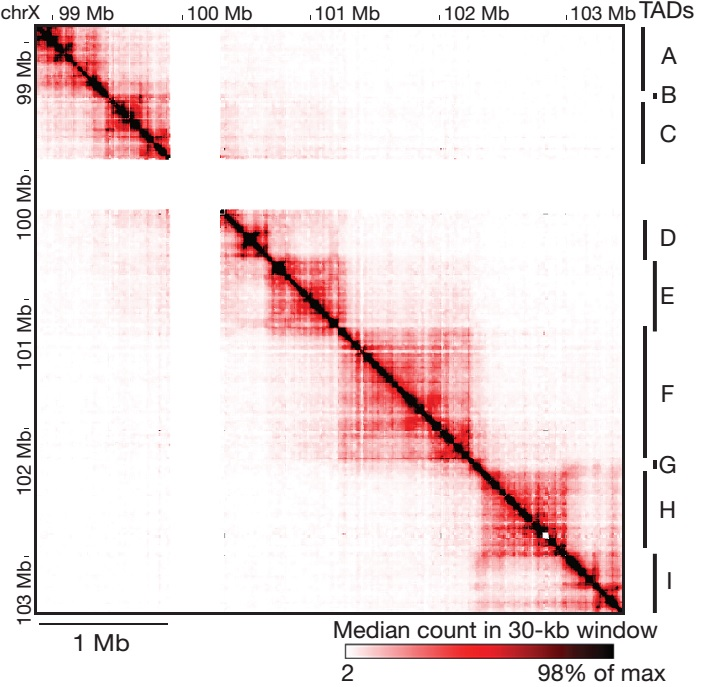
\includegraphics[scale=0.2]{TADsOfTheXChromosome_NoraEtAl2012}
\quad
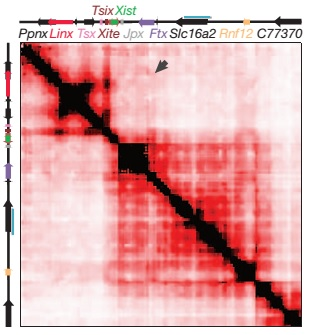
\includegraphics[scale=0.25]{TadDandENoraEtAl2012} 
\quad
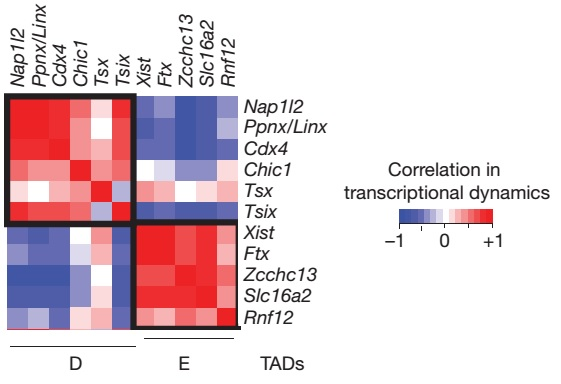
\includegraphics[scale=0.27]{transcriptionCorrelationTadDandENoraEtAl2012}
\caption{\tiny{The 4.5 Mb region (left), enlargement of TAD D and E (center). Displayed median count in a 30kb window every 6kb, gene expression Peasrsons correlation (right)}}
\label{fig:TADsOfTheXChromosome_NoraEtAl2012}
\end{figure}
\end{frame}

\section{Analysis of the data}\label{section_analysisOfTheData}

\begin{frame}{From restriction segments to beads}
\begin{itemize}
\item Coarse-graining of the data was made by choosing a bead-size of 3000 bp, corresponding to the mean segment length resulted from the digestion of HindIII. 

\begin{figure}[H]
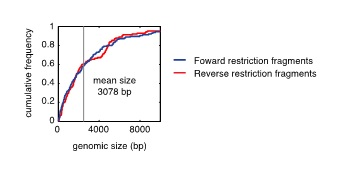
\includegraphics[scale=0.55]{restrictionSegmentLengthDistributionLucaetal}
\end{figure}
\item The genomic section was evenly partitioned. Each bead receives a start and end index according to the segment it covers. 
\item for example: 
\begin{tabular}[H]{|l| l| l|}
\hline
bp range & start ind & end ind\\
\hline
500-3500   & 1         & 2 \\
4000-4500  & 2         & 2 \\   
5000-12001 & 2         & 4 \\       
\hline  
\end{tabular}
\end{itemize}
\end{frame}

\subsection{TAD D and E}\label{subsection_tadDAndE}

\begin{frame}{Bead encounter frequecy}
\framesubtitle{TAD D and E}
\begin{itemize}
\item We work with the average of the two experimental replicates.
\item A total length of 920,432 bp - resulting in 307 beads (TAD D 107 beads, TAD E 200 beads).
\item We calculate the encounter probability as a function of distance (bead units) for each bead.
\item TAD E has several strong specific interactions. TAD D has weak intra long range interactions. Strong inter-TAD specific interactions
\end{itemize}

\begin{figure}[H]\label{TADDAndEencounterProb}
\centering
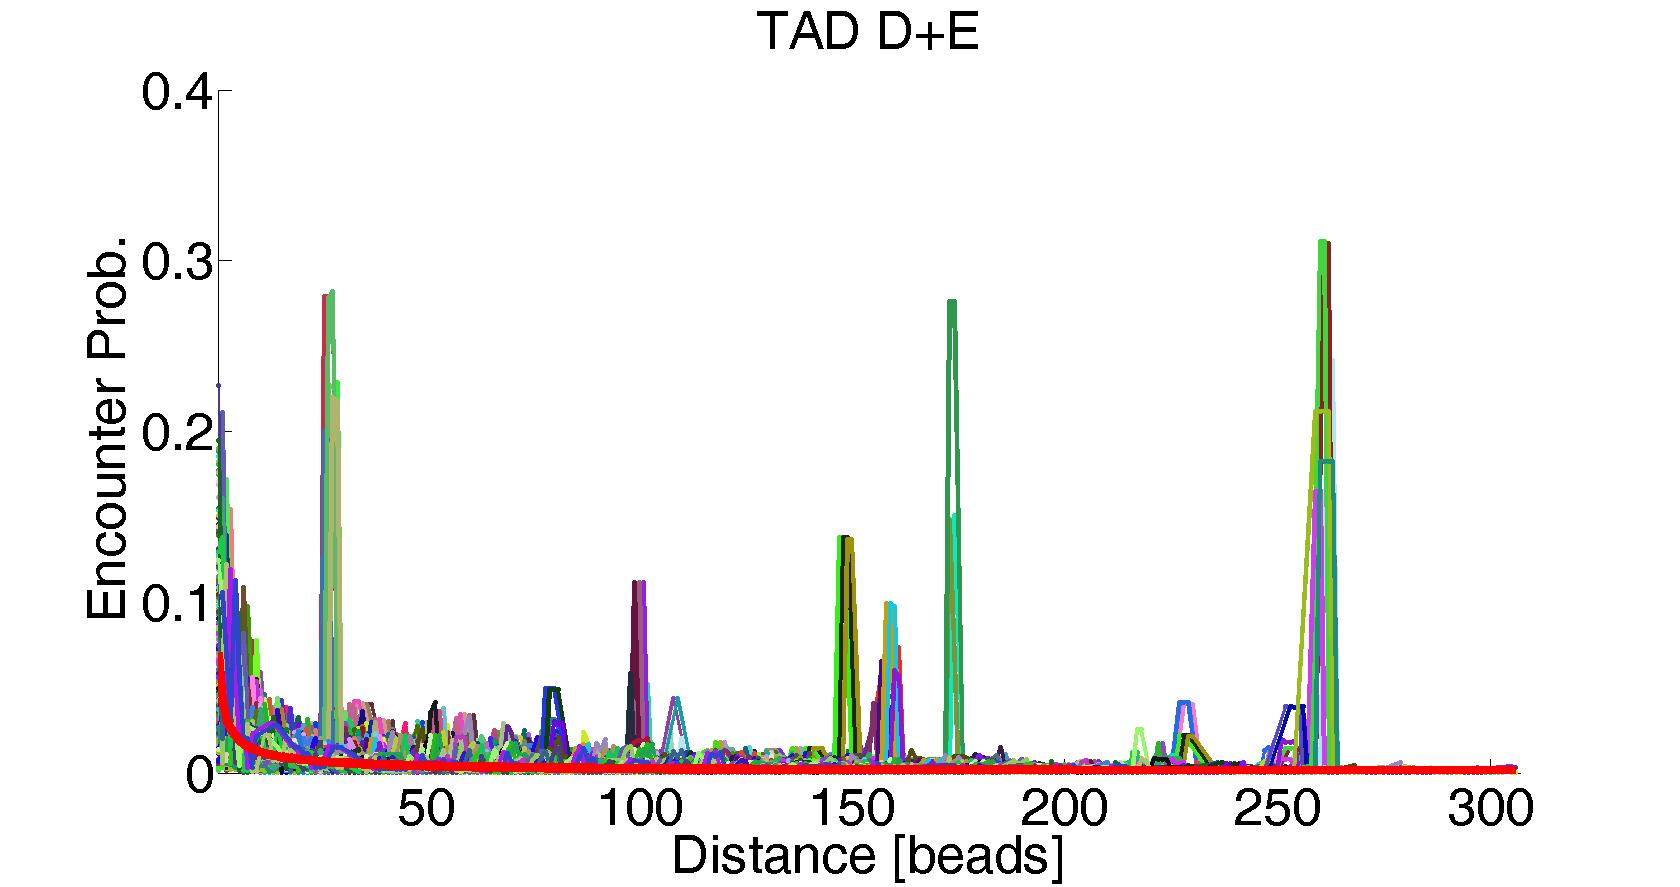
\includegraphics[scale=0.078]{encounterProbabilityTADDAndE}
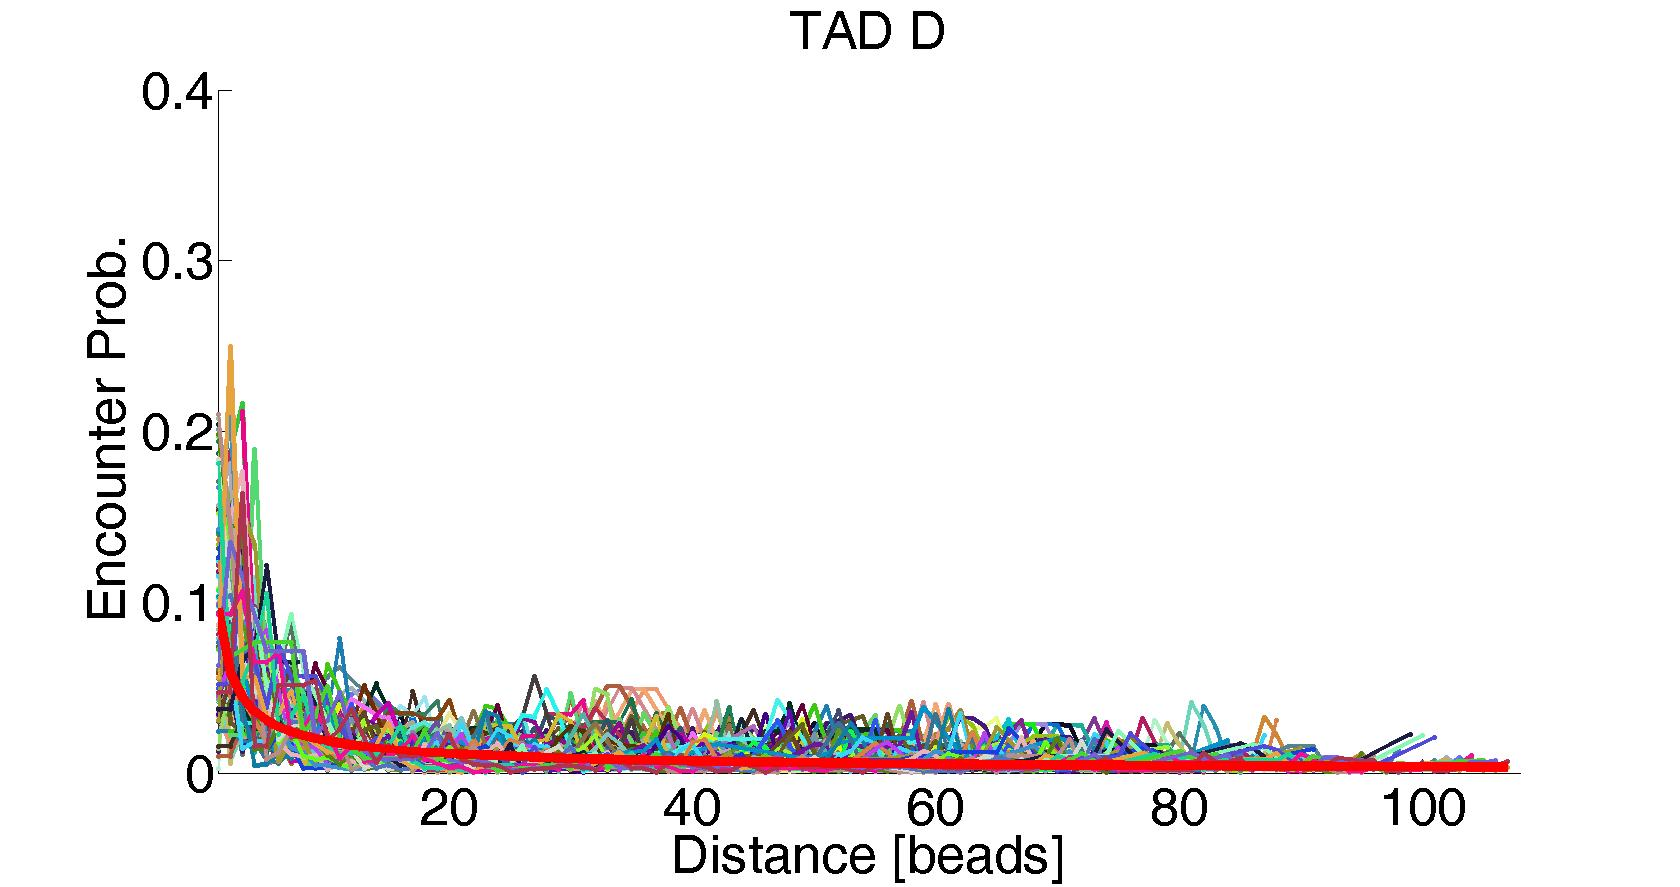
\includegraphics[scale=0.075]{encounterProbabilityTADD}
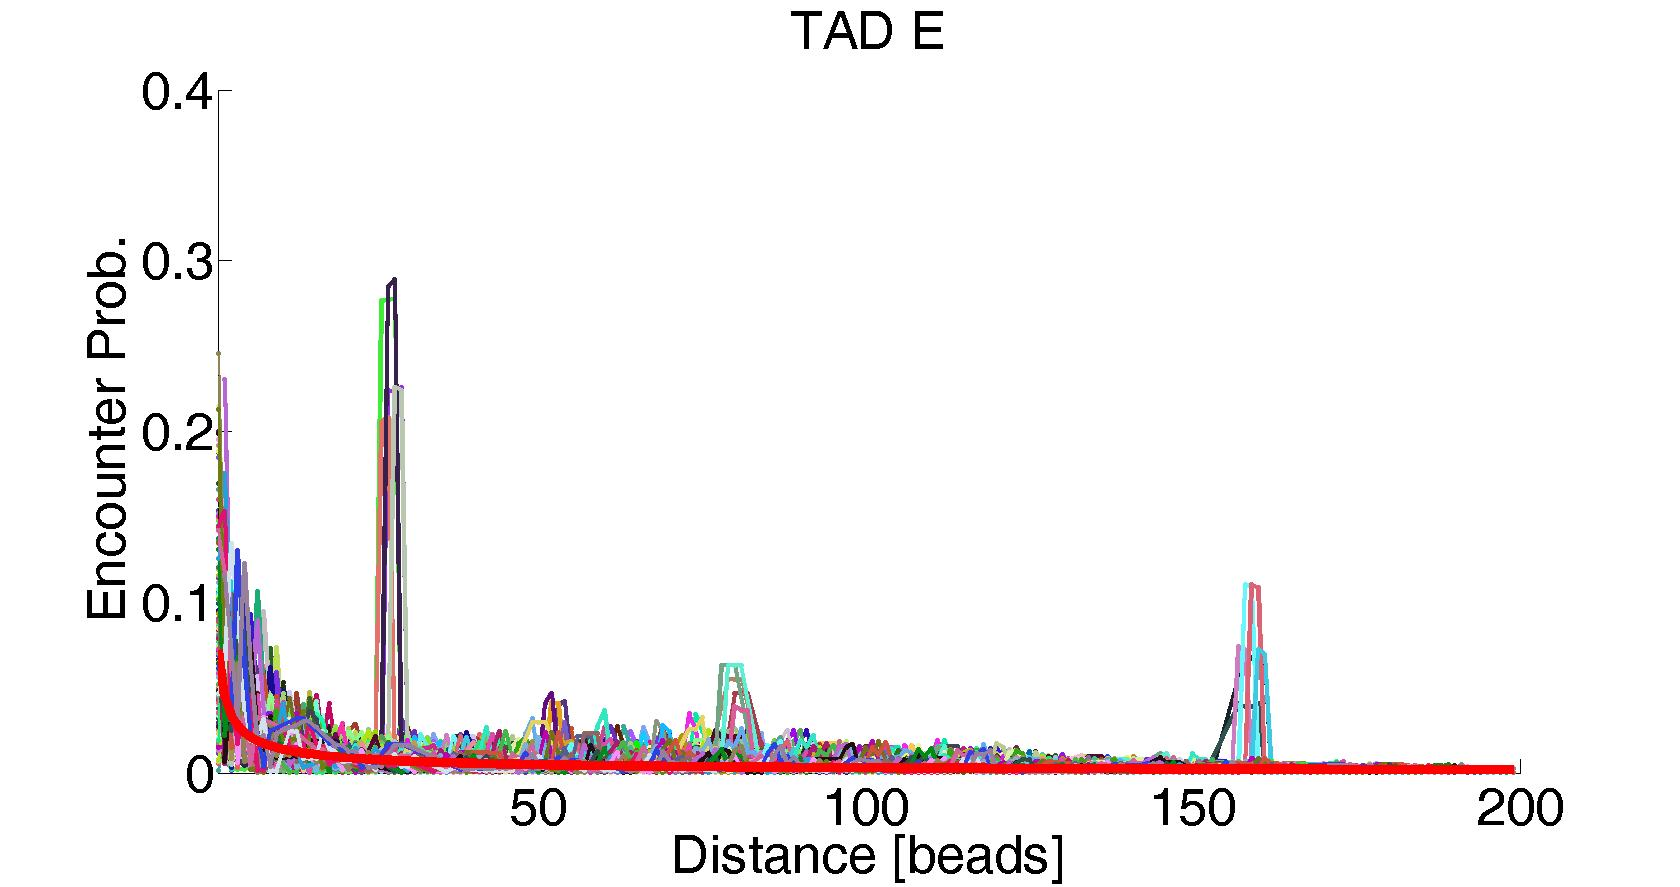
\includegraphics[scale=0.075]{encounterProbabilityTADE}
\end{figure}
\end{frame}

\section{Theoretical model}\label{section_theoreticalModel}

\begin{frame}{Theoretical model}
\framesubtitle{The Rouse model}
To understand the dynamical process underlying the observed encounter probabilities we need a employ a polymer model. We start with the classical and most simple model, the Rouse chain.
\begin{itemize}
\item A Rouse chain describes polymer dynamics as a stochastic motion of a collection of microscopic "beads" connected by harmonic springs
\item the 3D  motion of bead $n$ in the chain of $N$ beads 
\begin{equation*}
\frac{dR_n}{dt} = -\frac{3D}{b^2}(2R_n(t)-R_{n+1}(t)-R_{n-1}(t))+f_n(t)
\end{equation*}
\item $R_n$- the position of bead $n$\\
$b$- the standard deviation of the distance between adjacent beads\\
$D$- the diffusion constant\\
$f_n$- white Gaussian noise
\item From the theory, $Pr(\|R_n-R_m\|<\epsilon)\sim  |n-m|^{-1.5}$
\end{itemize}

\begin{figure}[H]
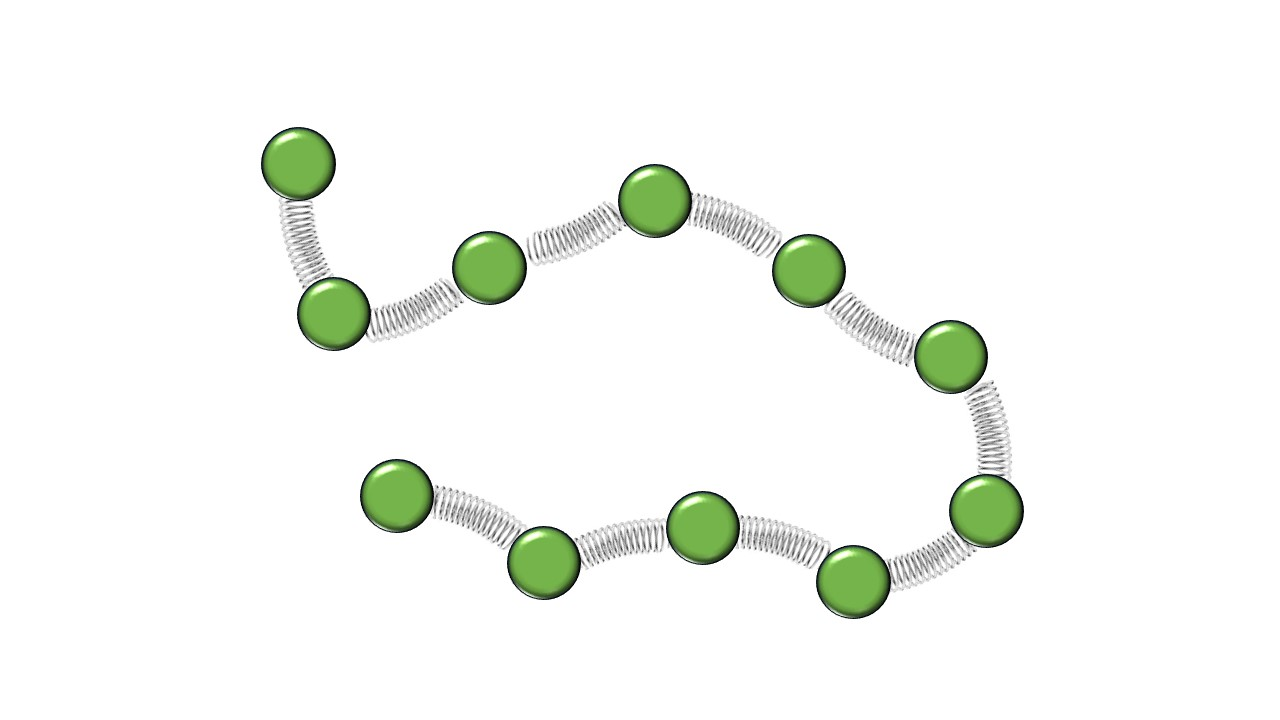
\includegraphics[scale=0.1]{RousePolymerSketch}
\end{figure}
\end{frame}

\subsection{The encounter probability}\label{subsection_theEncounterProbability}

\begin{frame}{The enconter probability}
For the case of TAD D, TAD E, and the two together, we estimate the bead encounter probability, $p$, and fit it with a function of the form 
\begin{equation*}
p_n(d)=\alpha d^{-\beta}
\end{equation*}
where, $d$ is the distance in [bead] units, $n$ is the bead number, $\alpha=\frac{1}{\sum_{j=1}^{d_{max}}j^{-\beta}}$ and $\beta$ is a parameter to be estimated.
We report the values of $\beta$ for each bead in each case.
\begin{figure}[H]
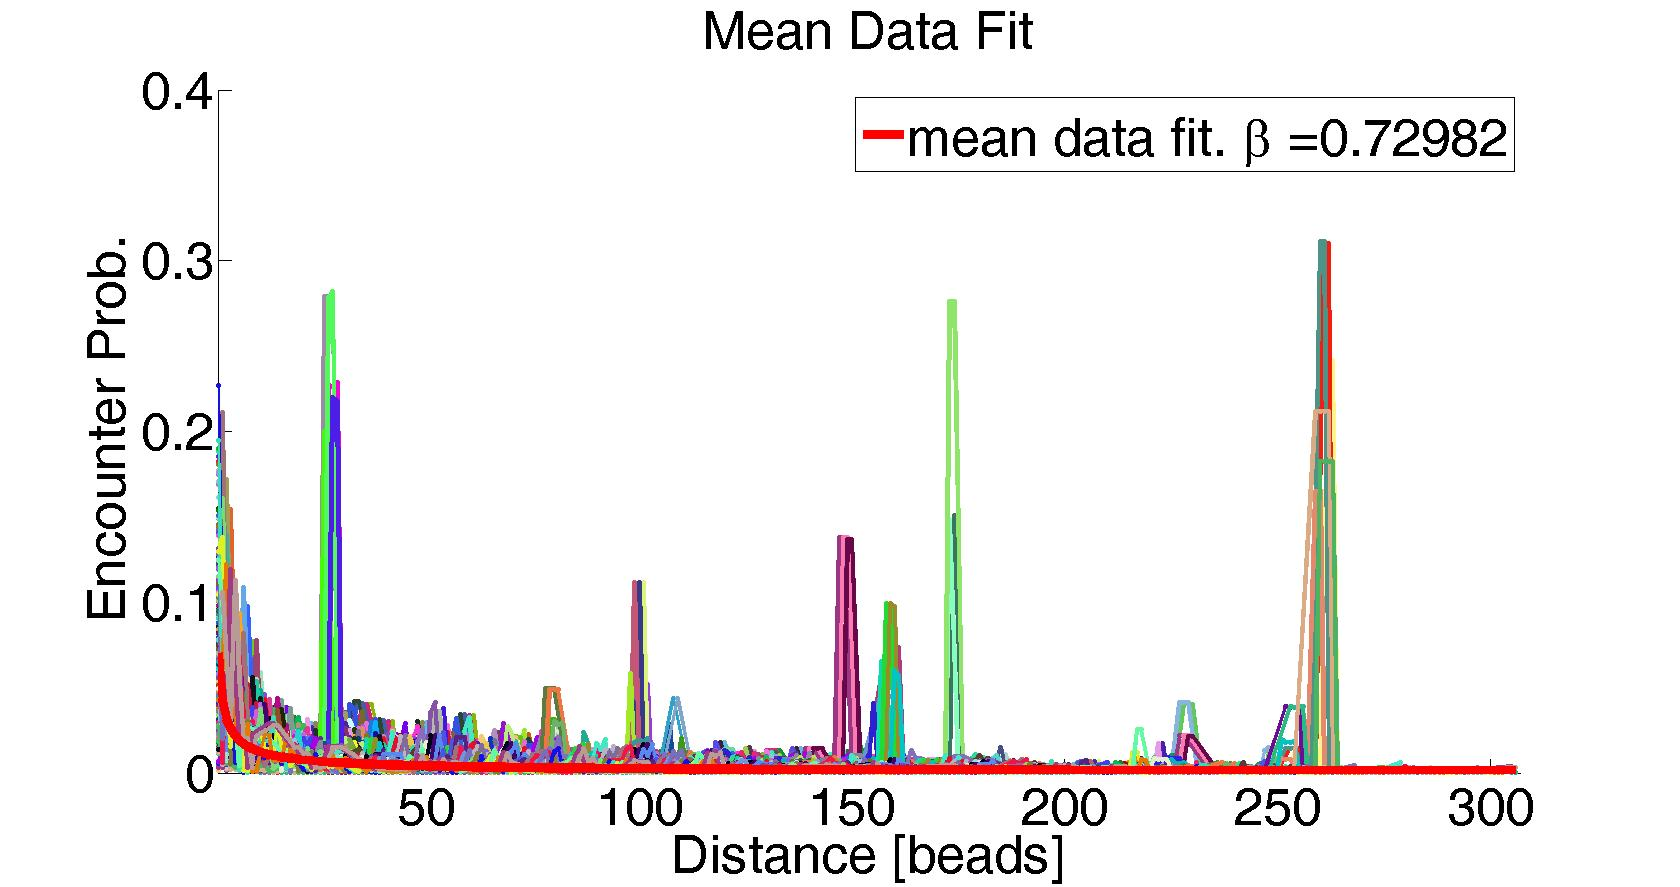
\includegraphics[scale=0.1]{meanDataFitTADDAndE}
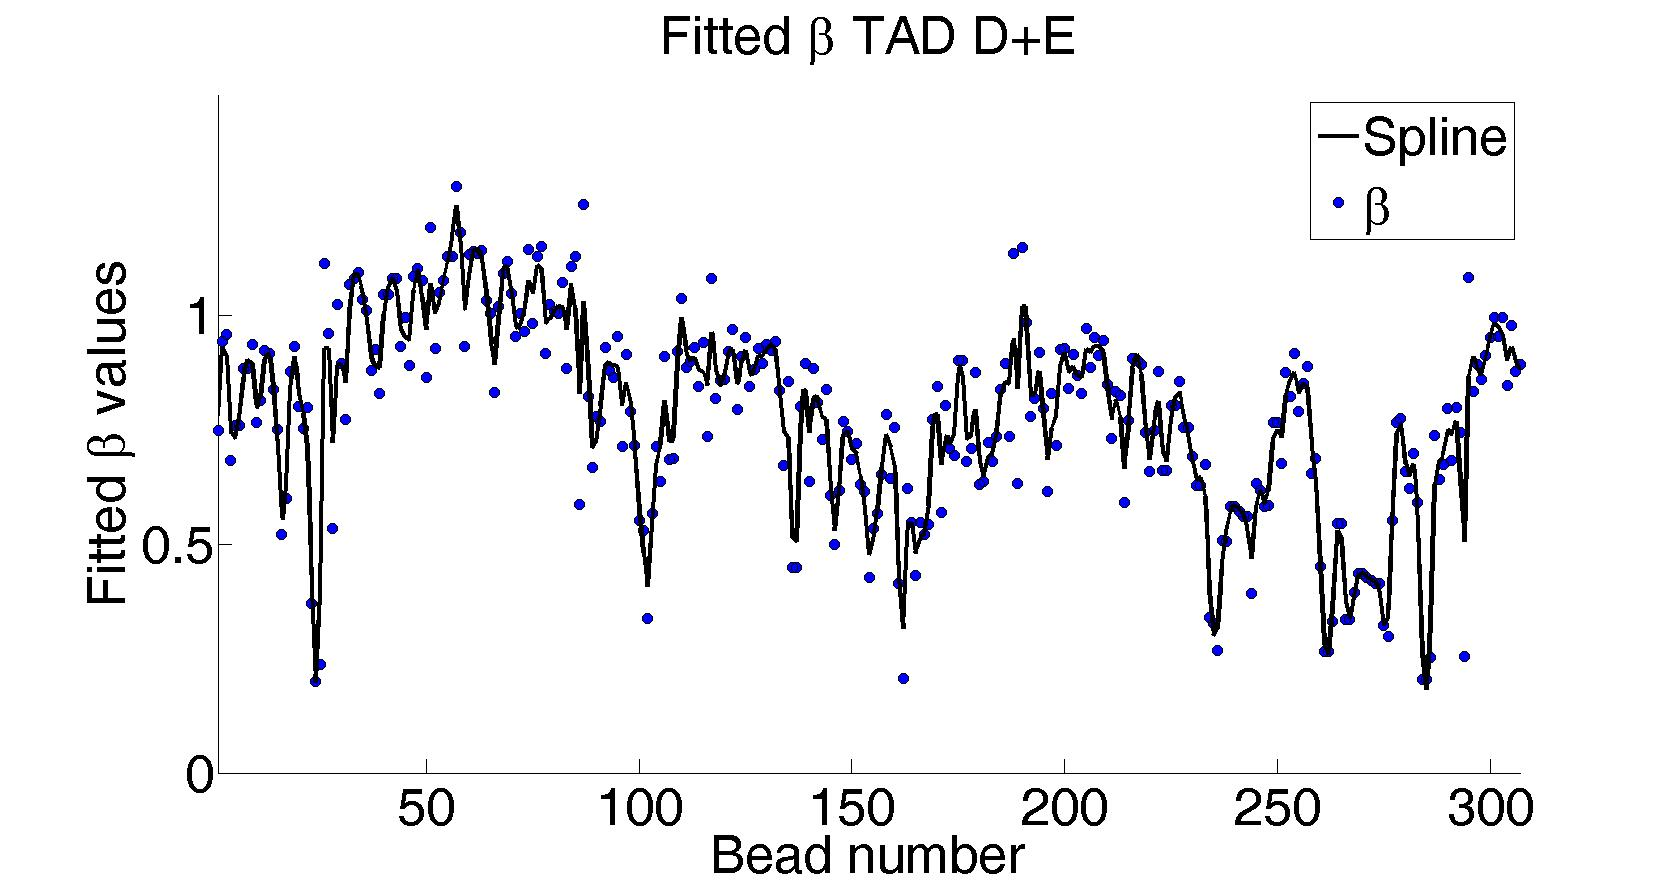
\includegraphics[scale=0.1]{fittedExpValuesWithSplineAverageTADDAndE}
\end{figure}
\end{frame}

\begin{frame}
\framesubtitle{TAD D and E}
\begin{figure}[H]
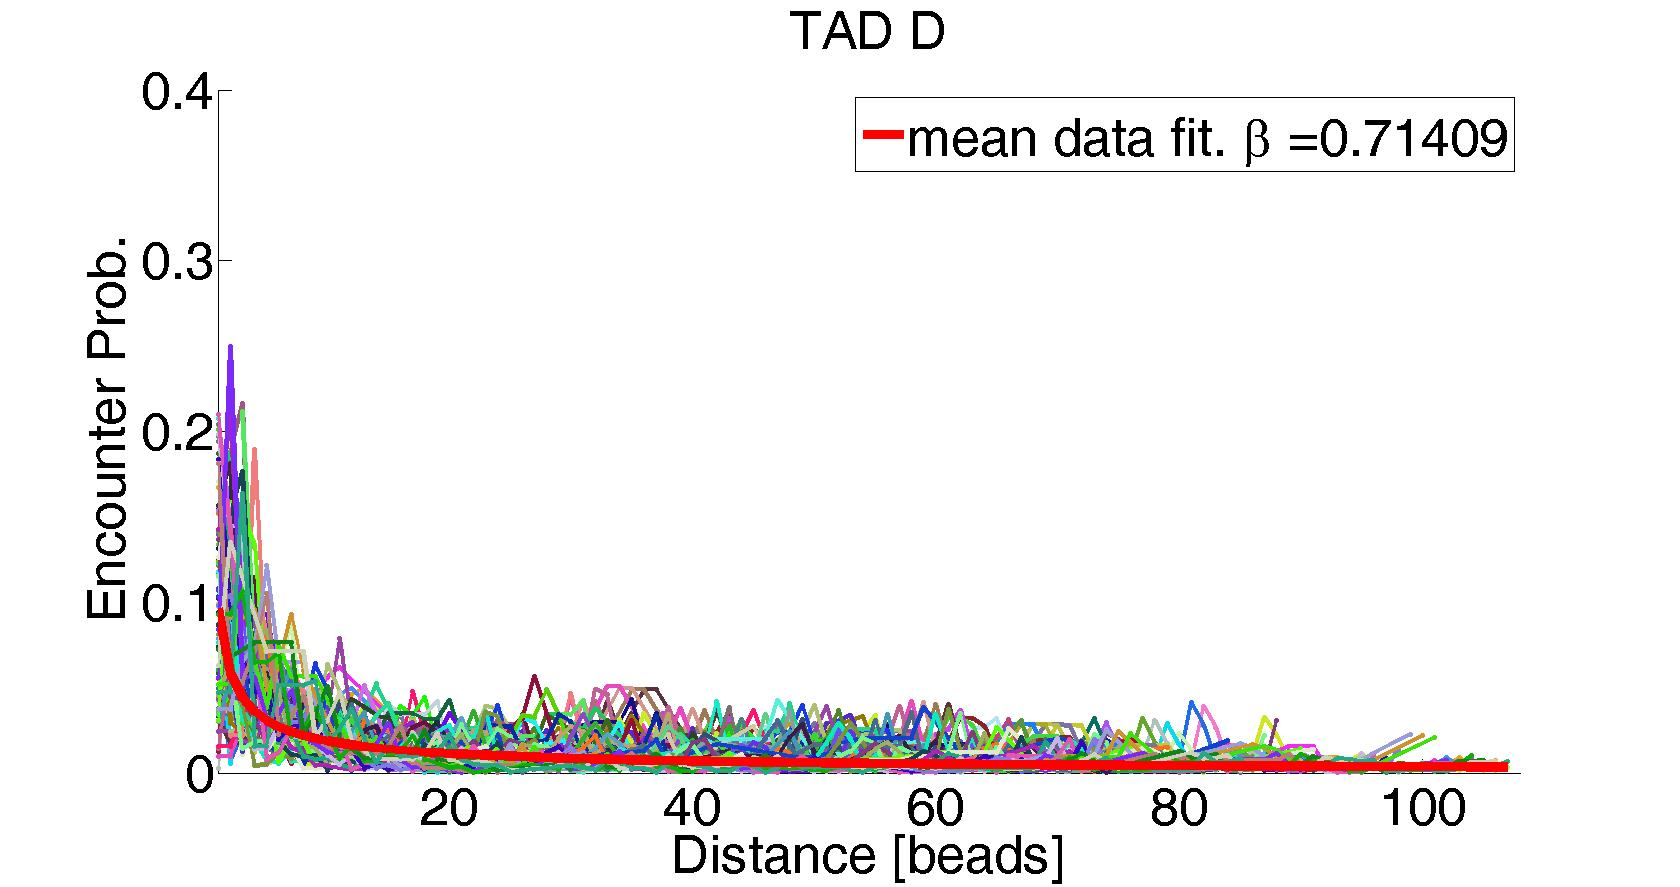
\includegraphics[scale=0.1]{meanDataFitTADD}
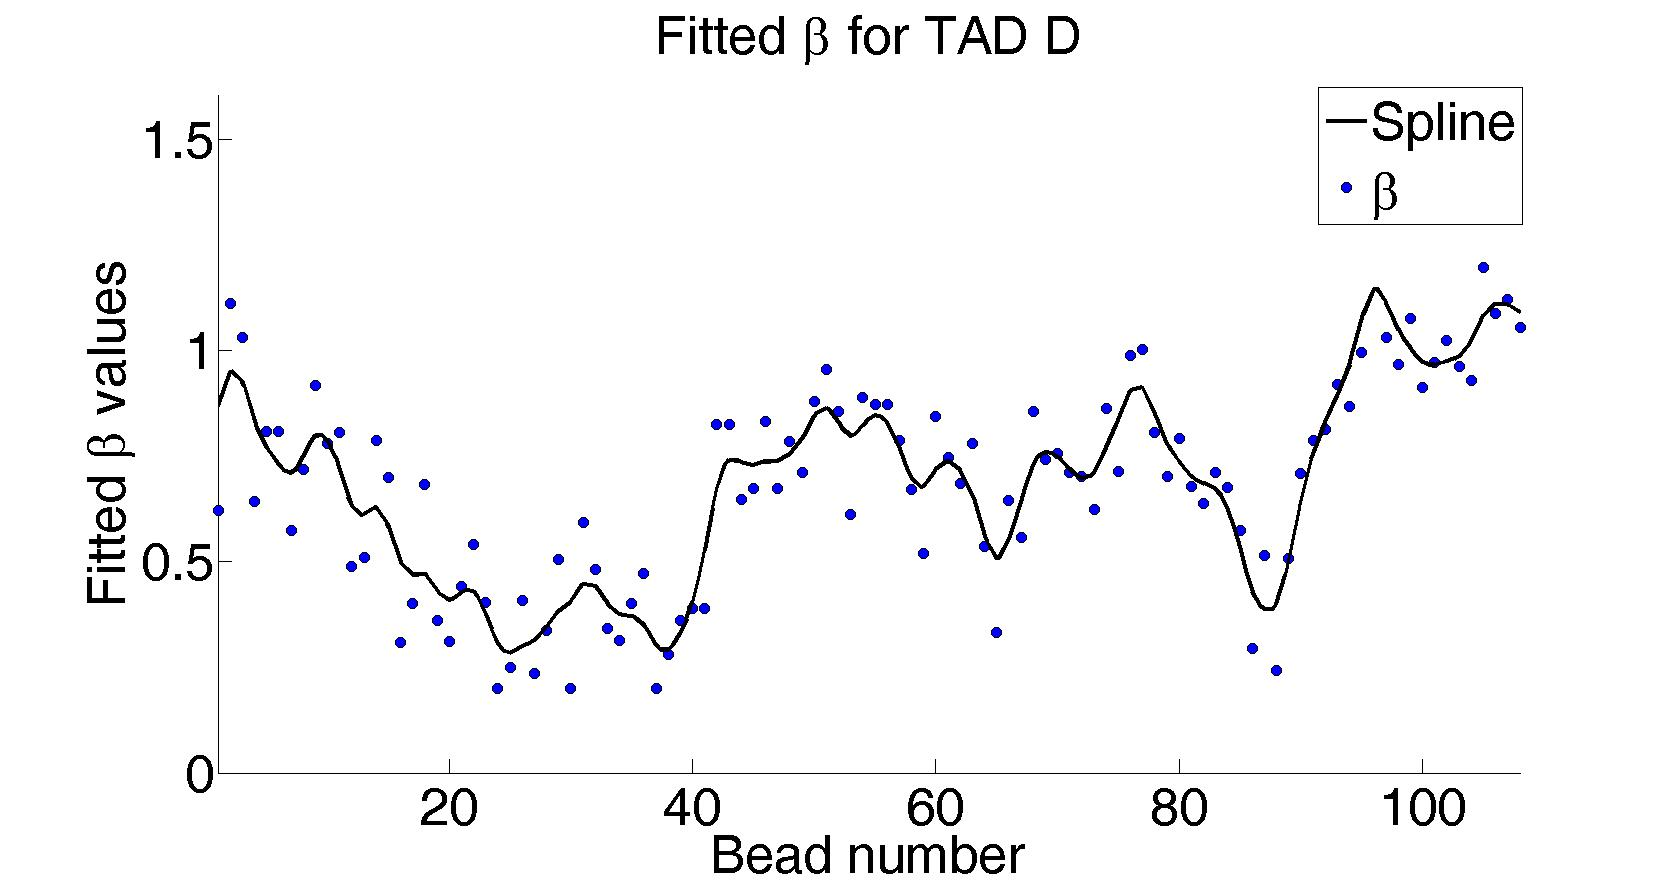
\includegraphics[scale=0.1]{fittedExpValuesWithSplineAverageTADD}
\end{figure}

\begin{figure}[H]
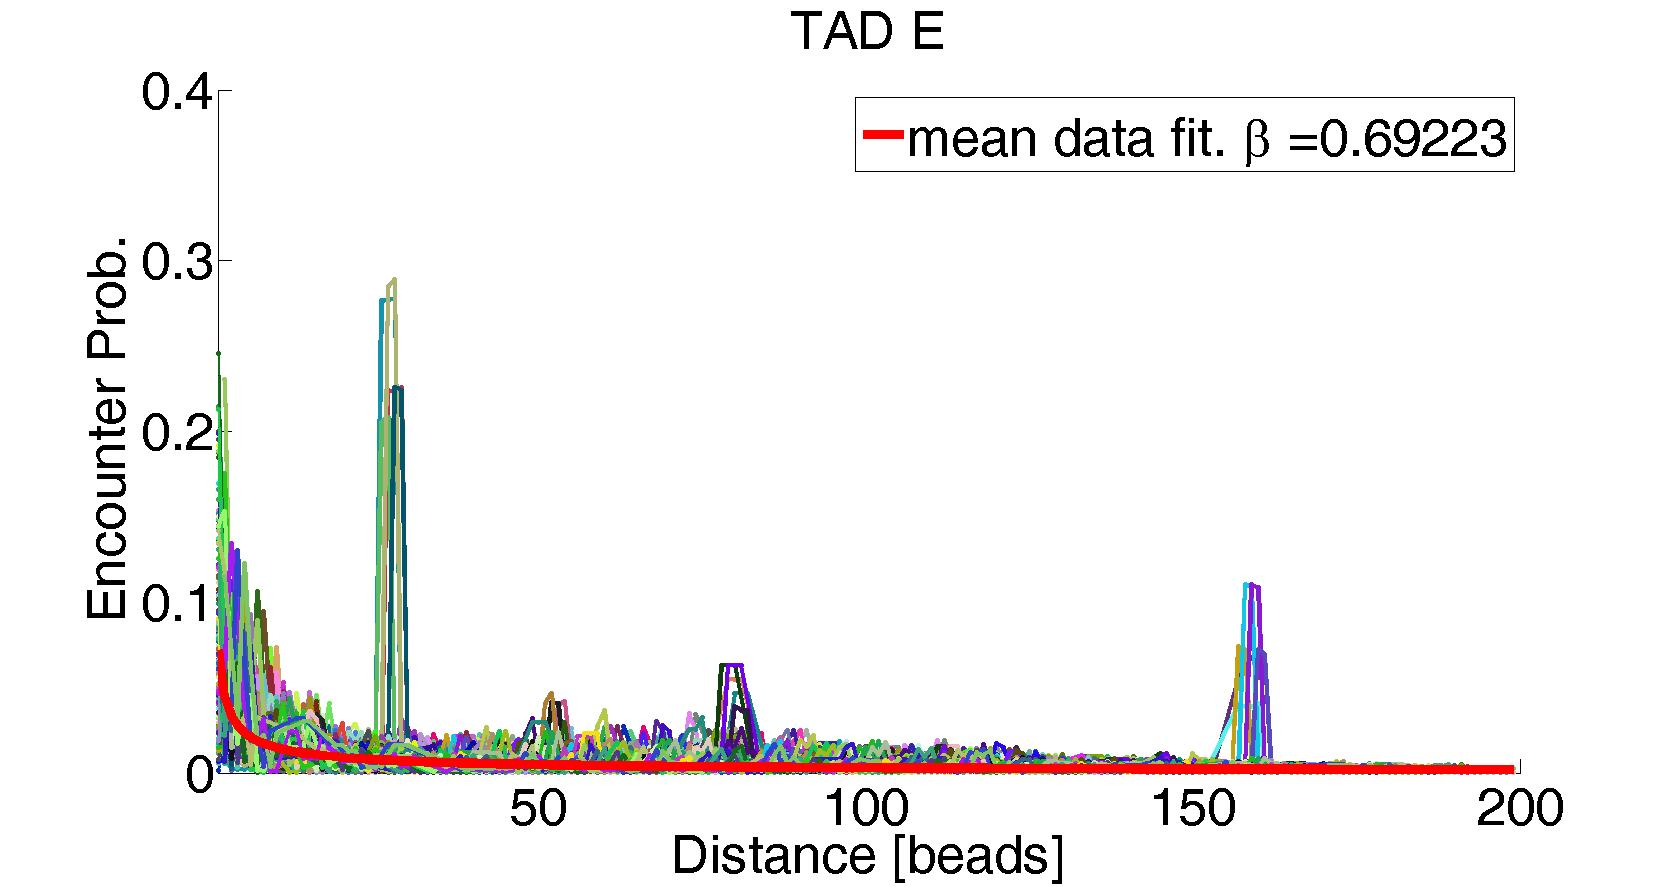
\includegraphics[scale=0.1]{meanDataFitTADE}
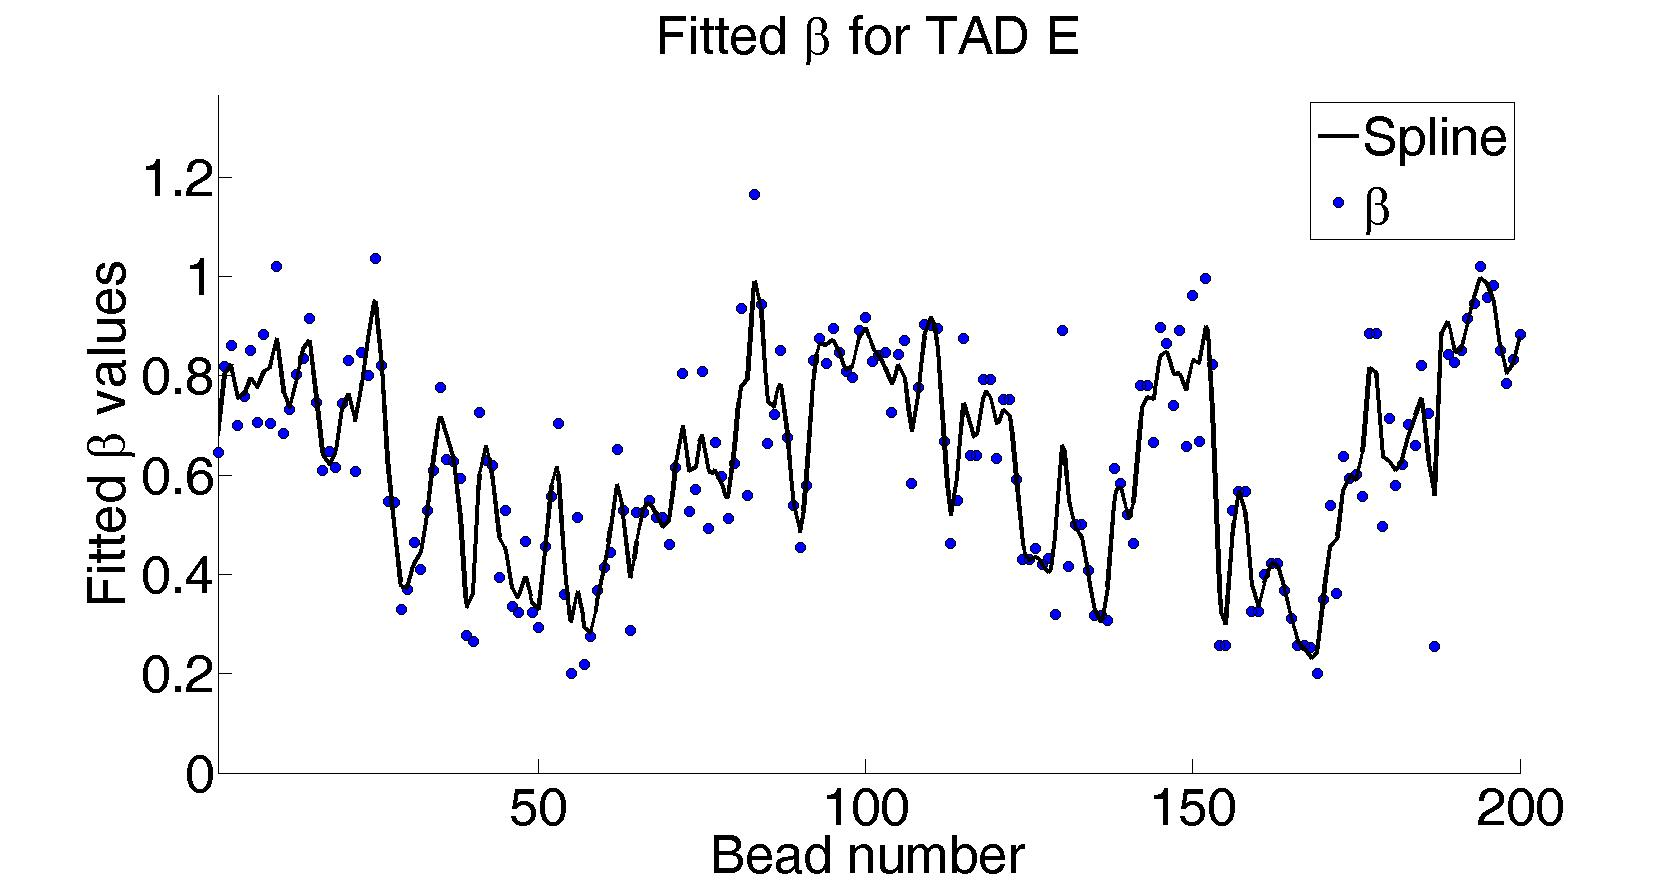
\includegraphics[scale=0.1]{fittedExpValuesWithSplineAverageTADE}
\end{figure}
\end{frame}

\subsection{Peaks of the encounter data}\label{subsection_peaksOfTheEncounterData}

\begin{frame}{Peaks of the encounter data}
\begin{itemize}
\item A peak-calling procedure was implemented to find pairs of beads which interact frequently. 
\item Peak analysis was performed separately for TAD D, E and between TADs. 
\item About $90\%$ of the peaks in the encounter data result from specific interactions between TADs and in TAD E.
\end{itemize}
\begin{figure}[H]
\includegraphics[scale=0.15]{peakListAverage}
\end{figure}

\end{frame}

\section{Simulation Results}\label{section_simulationResults}
%simulation section order:
% 1. normal Rouse 
% 2. normal rouse with peaks
% 3. rouse with random loops one TAD with tails 
% 4. rouse with random fixed loops in two TADs

\subsection{Simulations with a simple rouse chain}

\begin{frame}{Simulation with simple rouse chain}
\begin{itemize}
\item A simple Rouse model cannot reproduce the TAD, as expected.
\item Placing loops corresponding to the peaks of the encounter data does not reproduce the TADs. 
\end{itemize}
\begin{figure}[H]
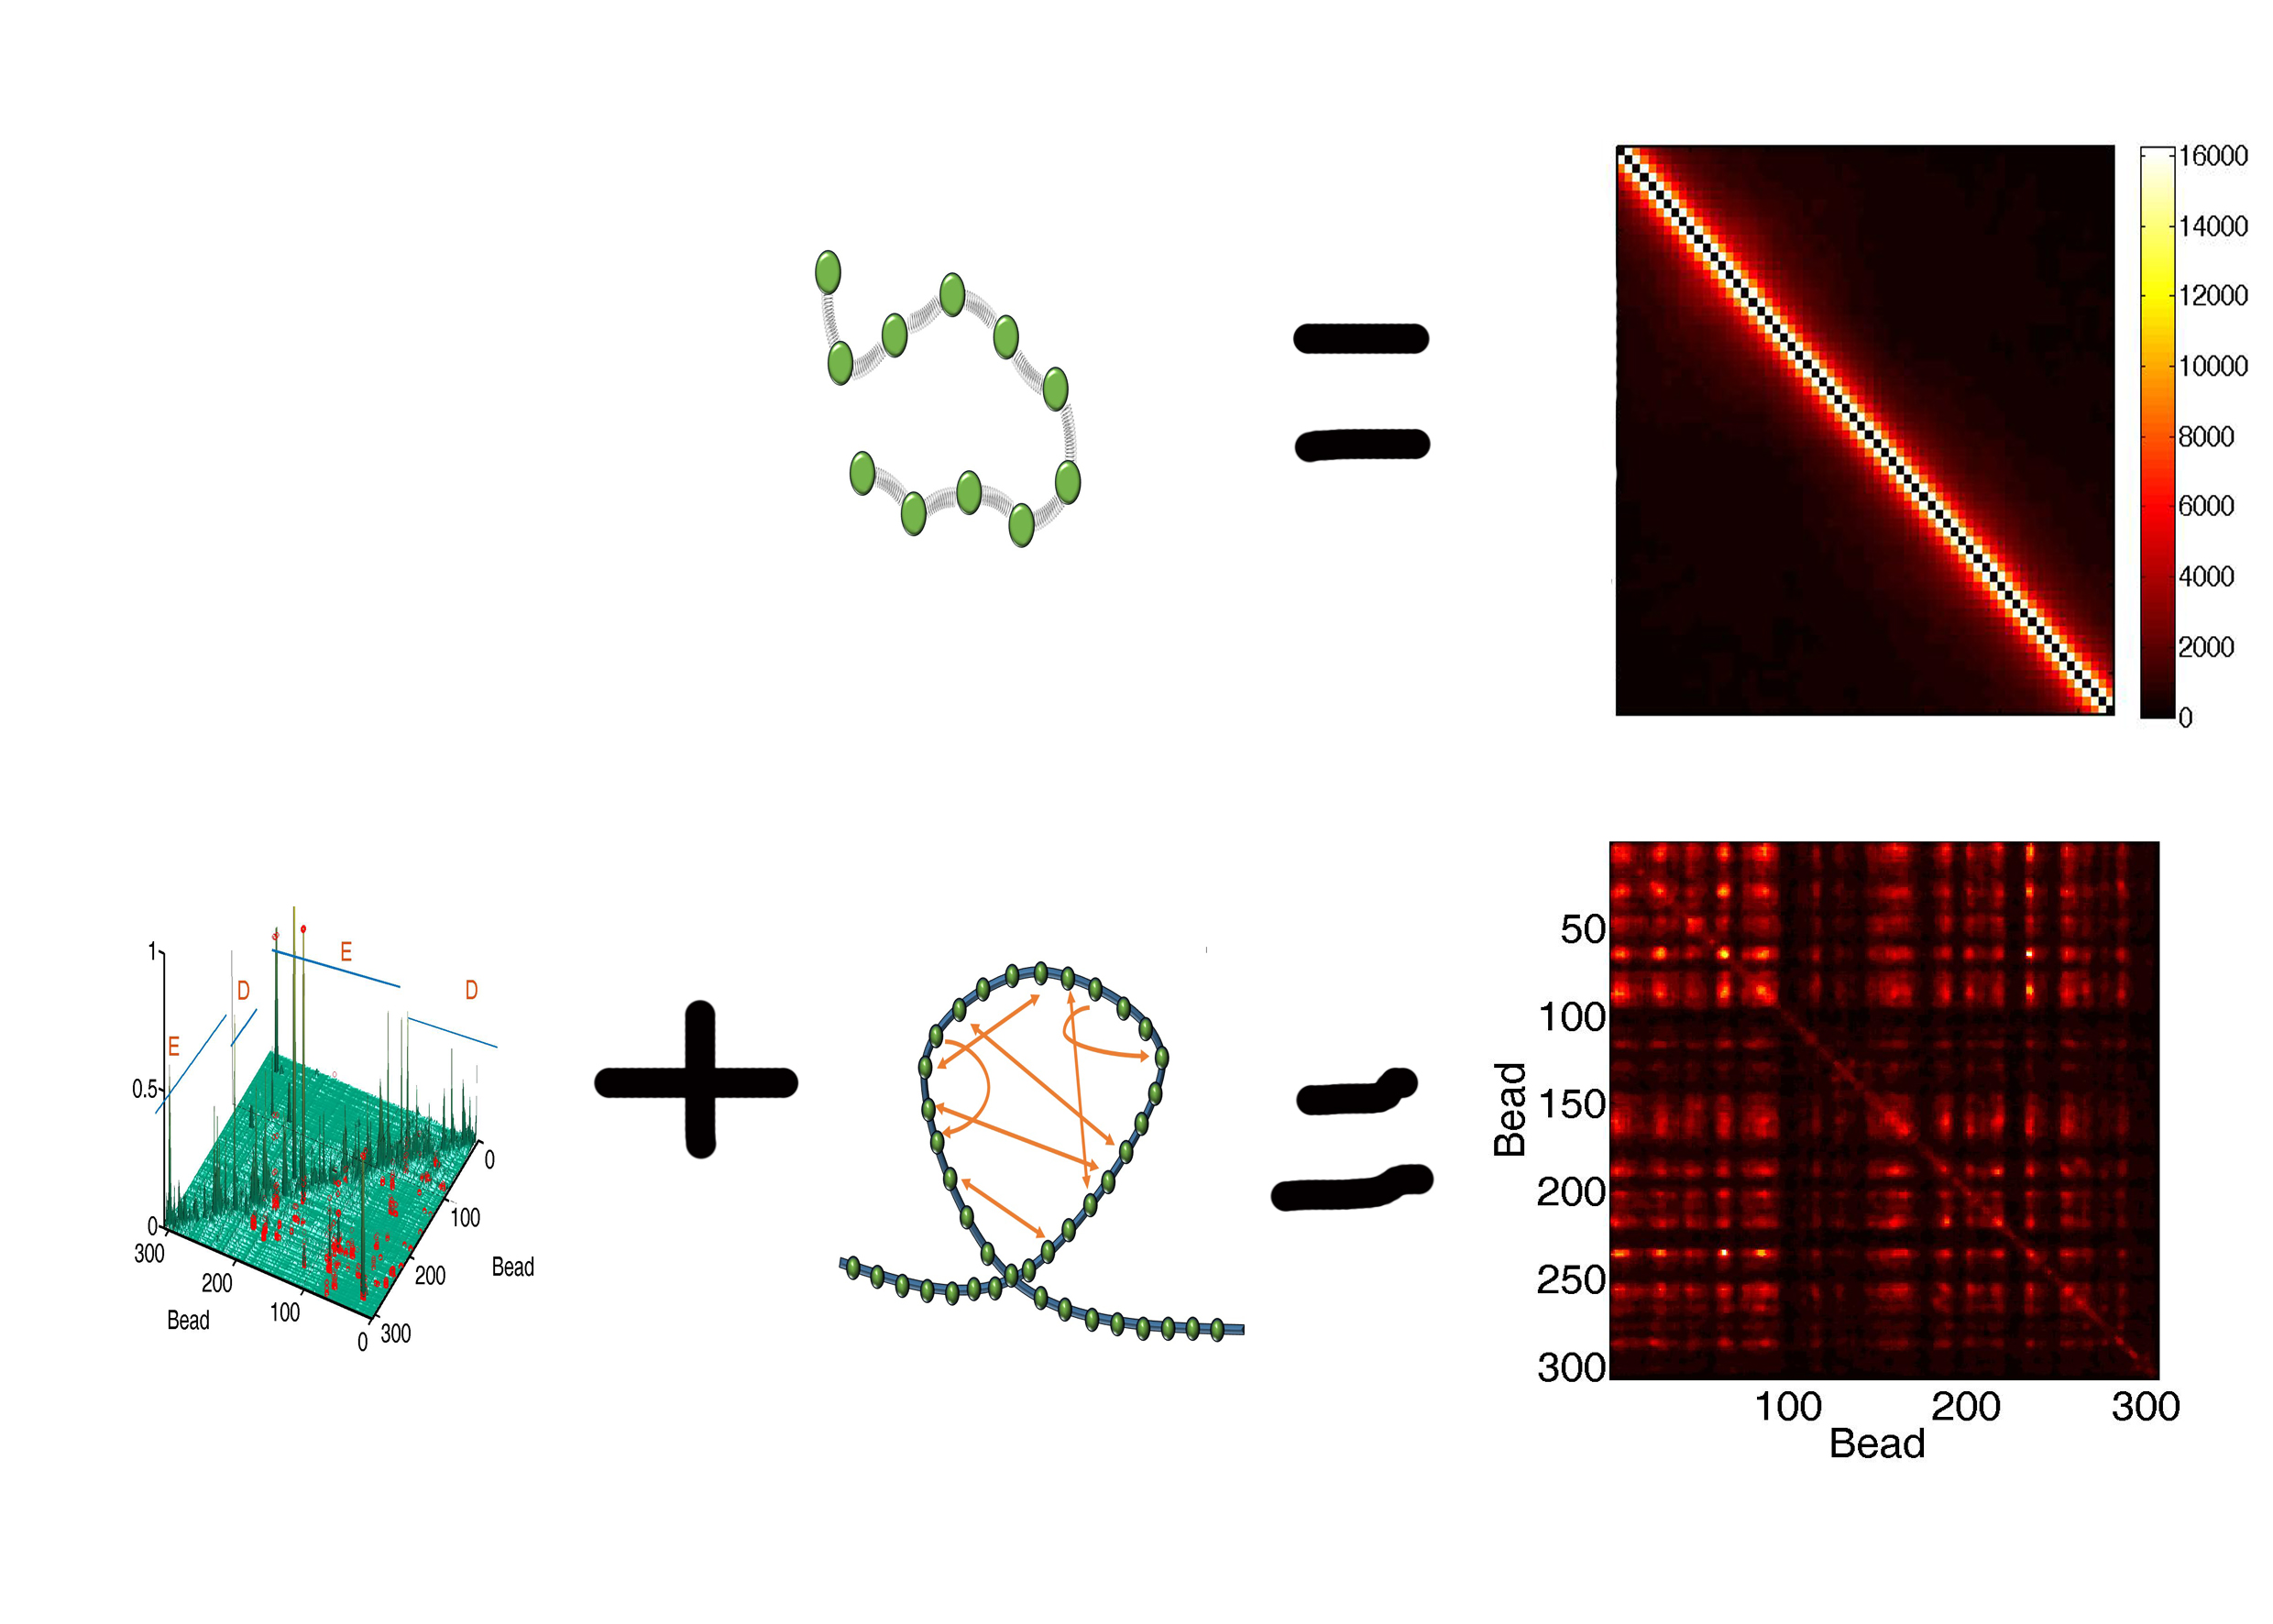
\includegraphics[scale=0.4]{simulationWithSimpleRouseExperimentalData}
\end{figure}
\end{frame}

\subsection{Random loops model}\label{subsection_randomLoopsModel}

\begin{frame}{Random Fixed Loop Model}
\begin{itemize}
\item The enhancer-transcription factor elements' encounter motivates the simulation of a chain with randomly placed loops.
\item These encounters might not be as frequent as 'stable' loops in the chromatin and therefore not shown significantly in the encounter maps.
\item Simulate a chain of 64 beads, having a random loop in a bounded region.
\item Increasing number of loops at random positions. 
\end{itemize}

\end{frame}

\begin{frame}{Stable loop with random loops within}
\framesubtitle{one TAD with 'tails'}
\begin{enumerate}
\item Following the peaks observation, we form a mix of 'stable' big loop with internal random loops.
\item In a 307 beads chain, beads 1075 and 207 were connected.
\item We iteratively add 30 connectors within the stable big loop.
\item We can start seeing the emergence of $\beta$ curve pattern as in the experimental data.
\end{enumerate}
\begin{figure}[H]
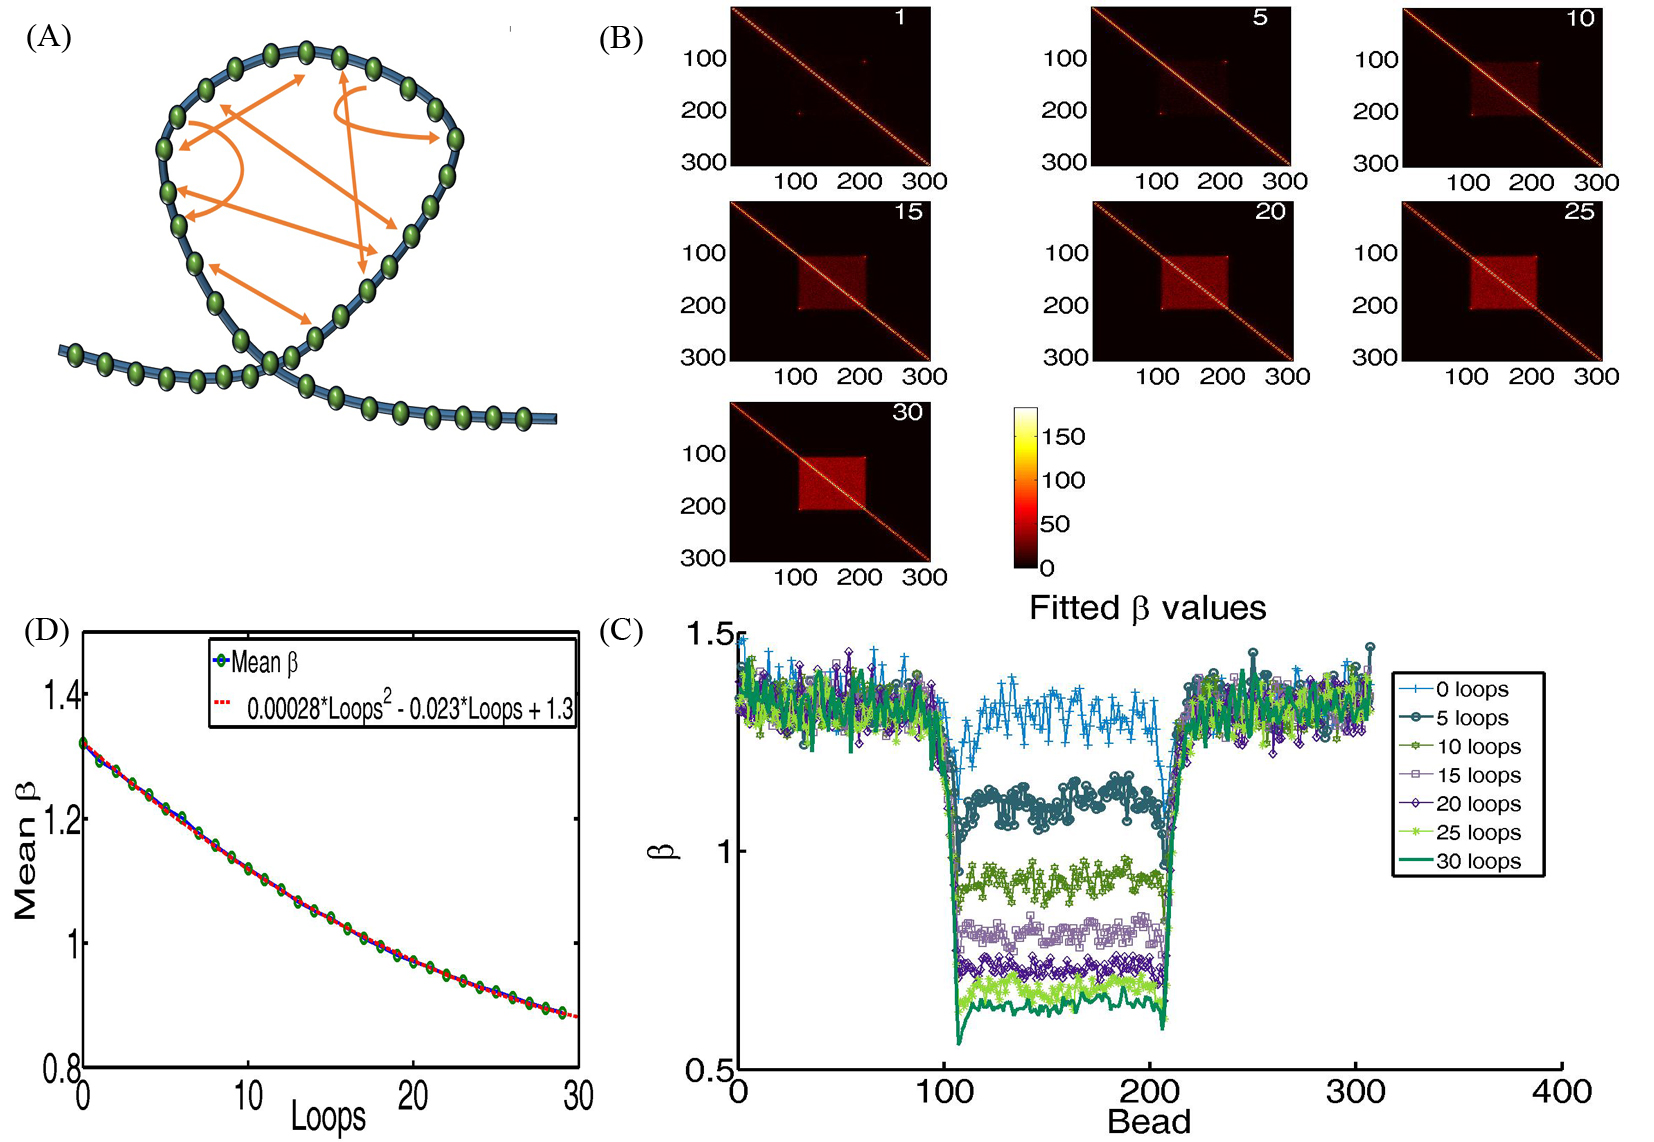
\includegraphics[scale=0.35]{Figure03_OneTADWithTails0To30RandomLoops}
\end{figure}
\end{frame}


\begin{frame}{Stable loop with random loops within}
\framesubtitle{Two TADs}
\begin{enumerate}
\item In a 307 beads chain, we create two stable loops by connecting bead 1 and 107, and bead 108 and 307
\item We iteratively add 30 connectors within TAD.
\item We can start seeing the emergence of $\beta$ curve pattern as in the experimental data.
\end{enumerate}
\begin{figure}[H]
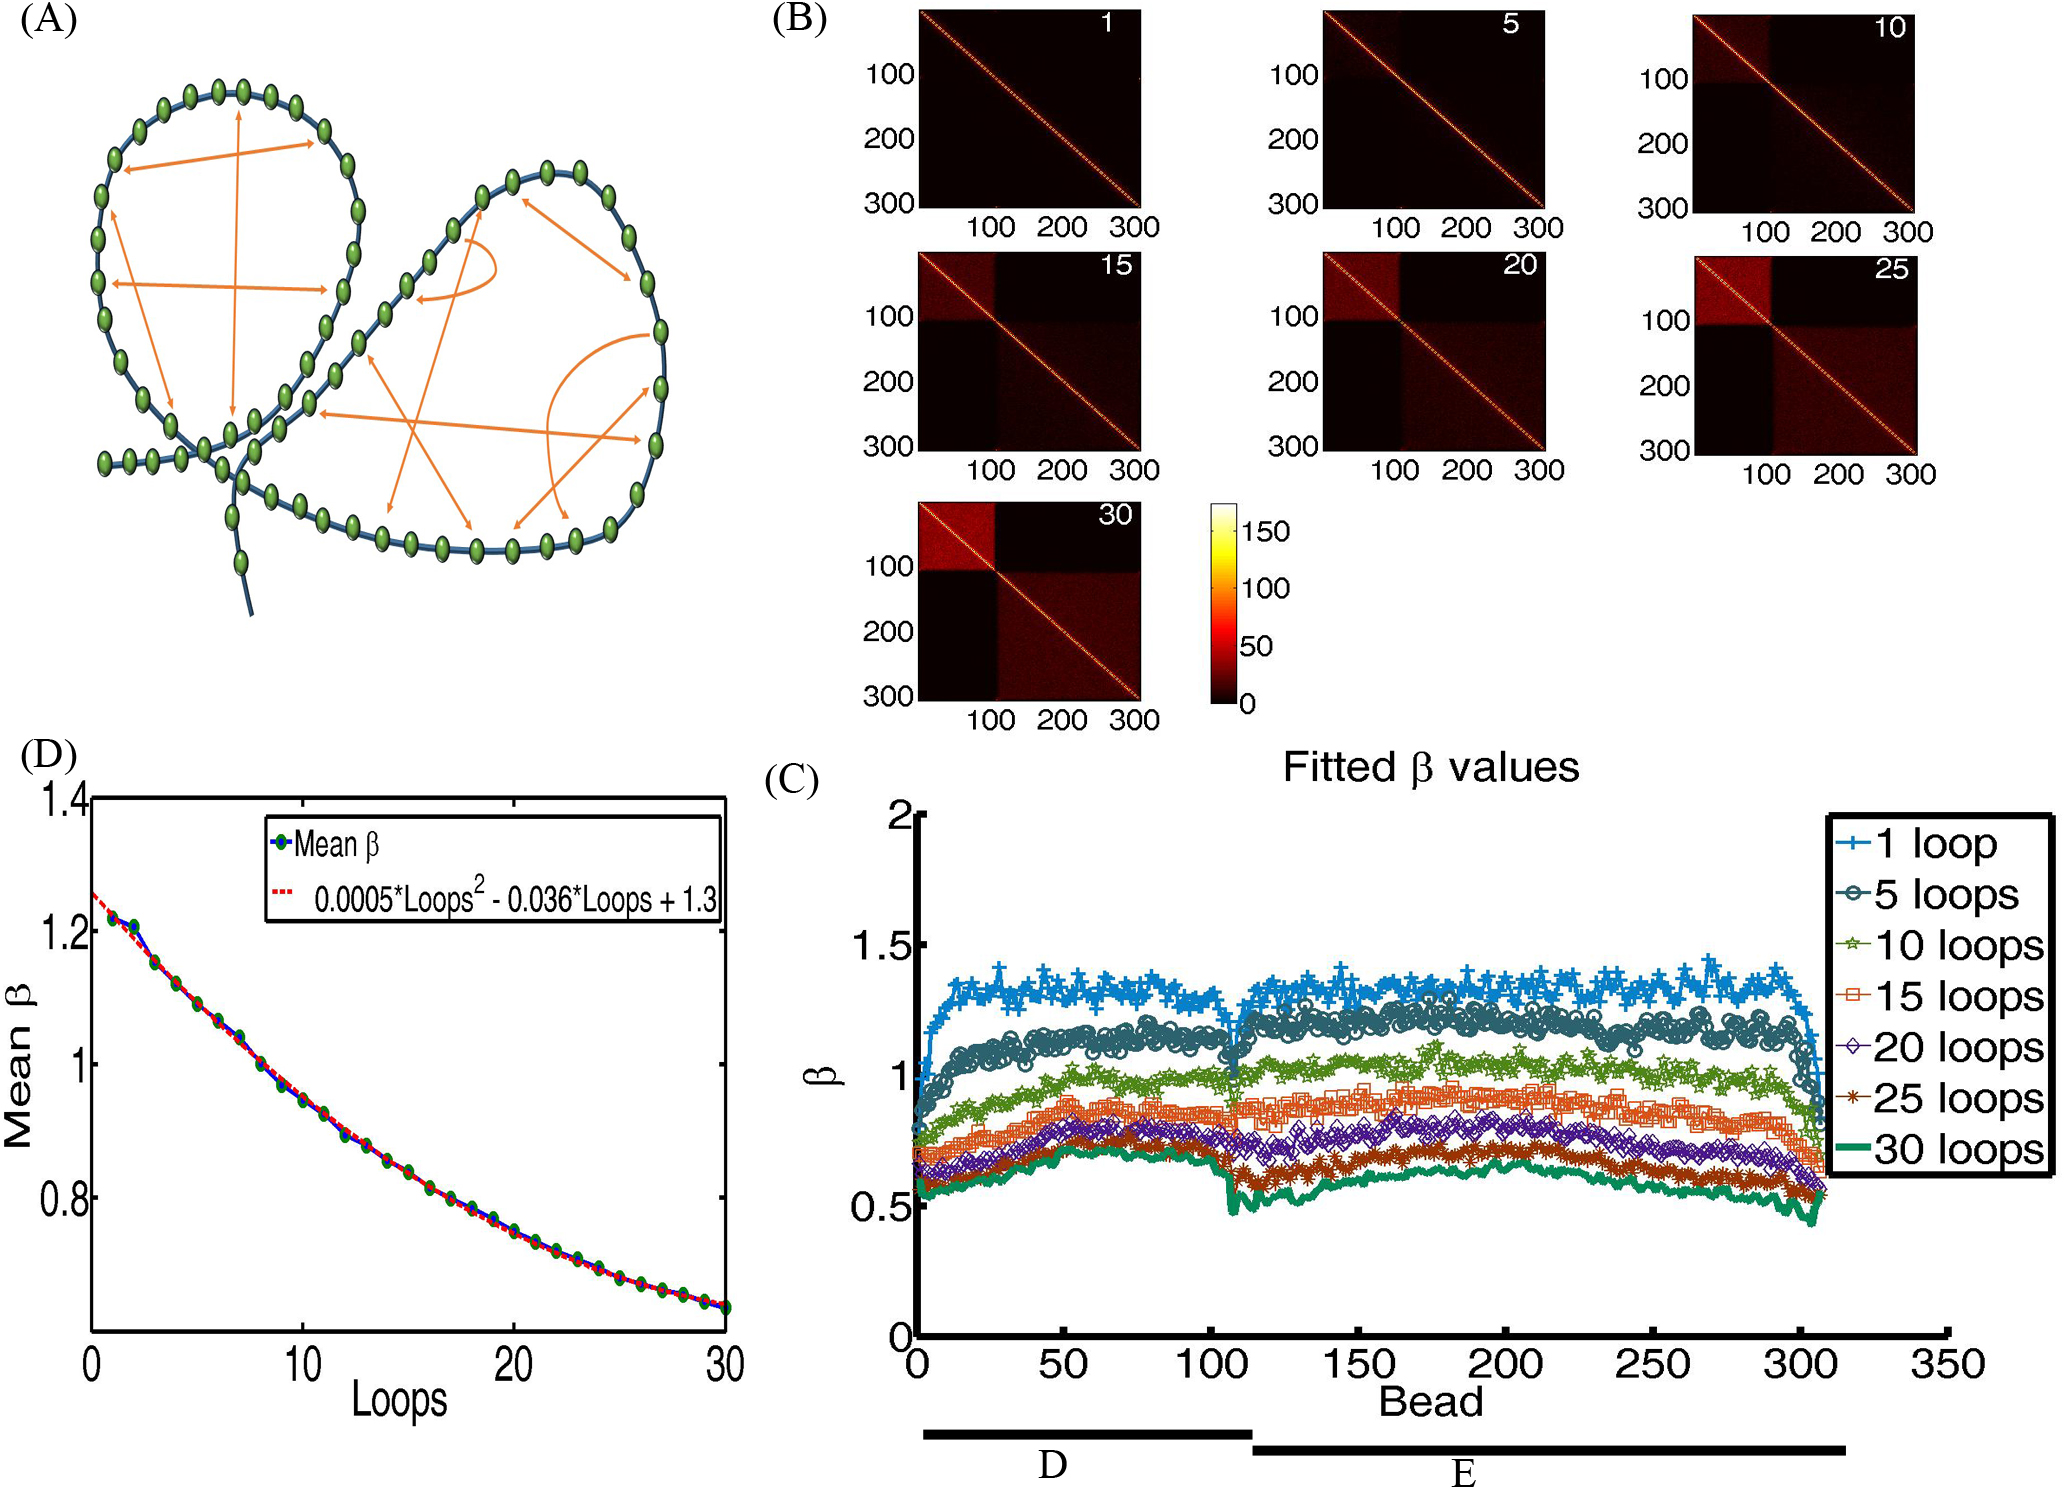
\includegraphics[scale=0.35]{Figure04_TwoTADs0To30RandomLoops307Beads}
\end{figure}
\end{frame}


\section{Summary}\label{section_summaryAndFutureWork}

\begin{frame}{Summary}
\begin{itemize}
\item We presented a plausible and simple model to explain the appearance of the conserved TAD domains. 
\item the model represent the results obtained in the population level.
\item A relationship between the mean number of loops and the encounter probability was shown by simulations.
\item The parameter used for our analysis, namely $\beta$, can easily calculated by experimentalists. 
\end{itemize}
\end{frame}

\begin{frame}{Work in progress}
\begin{enumerate}
\item Calculation of the mean first encounter time between beads in the Rouse ring
\item Showing analytically the relationship between number of loops and decrease in $\beta$
\item Put in more rigorous form the relationship between the pattern of $beta$ and the mean observed chromatin structure.
\item Calculating the equilibrium distribution of the random loop model
\item Simulating a model with random dynamic loops, in which loops can form and dissociate.
\item Experiment with more realistic polymer models.
\end{enumerate}
\end{frame}

\end{document}